\documentclass[11pt]{article}
%\documentclass{book}
\usepackage[utf8]{inputenc}
\usepackage[T1]{fontenc}
\usepackage[french]{babel}
\usepackage[top=1.8cm, bottom=1.8cm, left=1.8cm, right=1.8cm]{geometry}
\usepackage[linktocpage,colorlinks=false]{hyperref}
\usepackage{graphicx}
\usepackage{epsfig}
\usepackage{amssymb}
\usepackage{amsmath}
\usepackage{array}
\usepackage{subfig}
\usepackage{multicol}
\usepackage{caption}
\usepackage{listings}
\usepackage{algorithm}
\usepackage{algorithmic}
\hypersetup{
    colorlinks=true,
    breaklinks=true,
    urlcolor=red,
}
\parskip=5pt

\title{\huge{\textbf Manuel d'utilisation}}
\author{AYOUB Pierre, BASKEVITCH Claire, BESSAC Tristan, \\
CAUMES Clément, DELAUNAY Damien, DOUDOUH Yassin}
\date{Mercredi 1 Juin 2018}

\begin{document}

\maketitle
\vspace{20em}
\begin{center}
\includegraphics{pictures/Application.png}\end{center}
\newpage

\tableofcontents

\newpage

\section{Installation et désinstallation}

\subsection{Installation sous Linux}

Deux choix sont possibles pour Linux :

\begin{itemize}
\item Taper sur le terminal git clone https://www.github.com/Heisenberk/StegX
\item cd StegX
\item mkdir build 
\item cd build
\item cmake ..
\end{itemize}

\hspace{1cm}
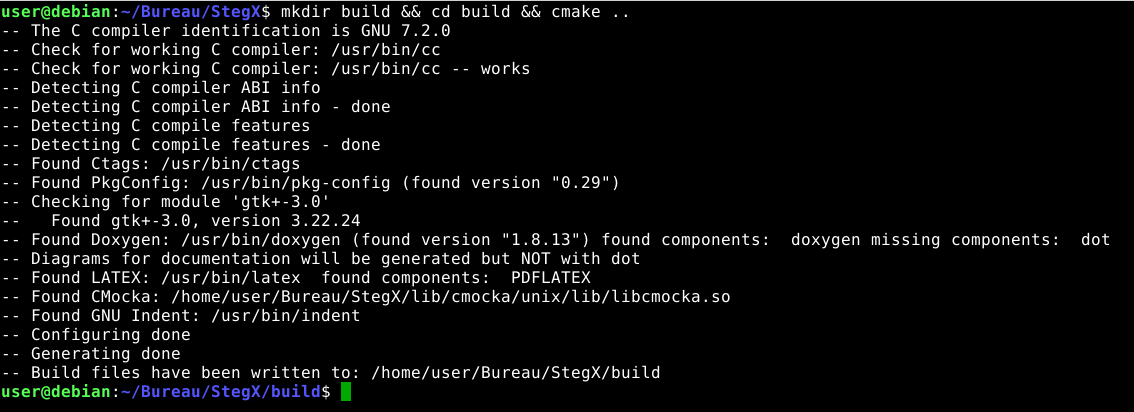
\includegraphics[scale=0.5]{pictures/build.png}
\vspace{0.5cm}

\begin{itemize}
\item make
\end{itemize}

\hspace{1cm}
\vspace{0.5cm}
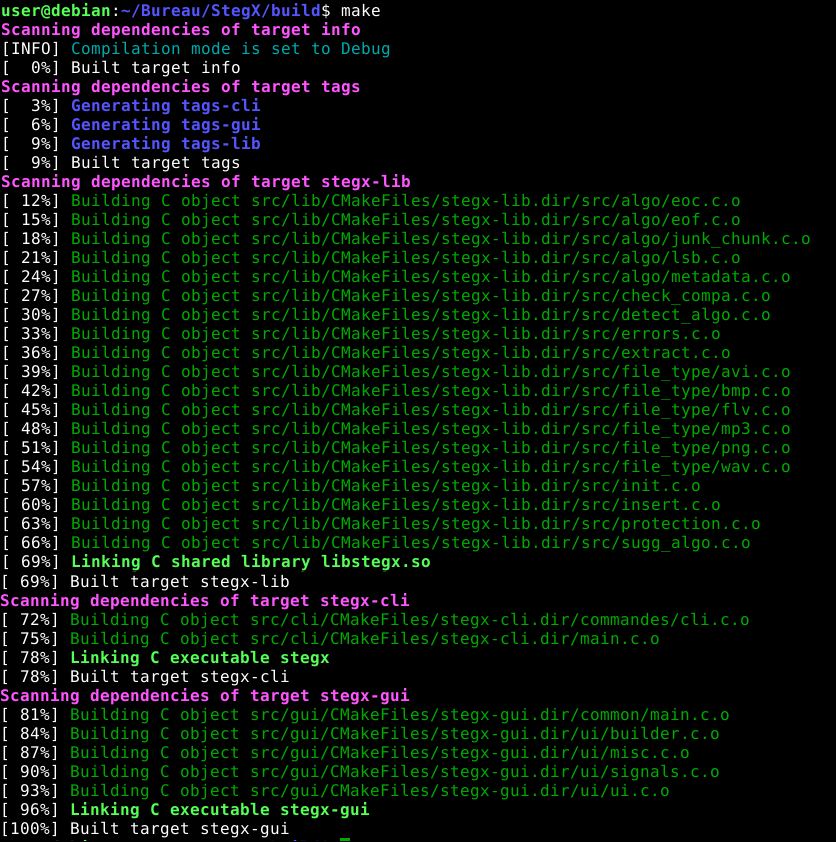
\includegraphics[scale=0.5]{pictures/make.png}


\begin{itemize}
\item sudo make install
\end{itemize}

\hspace{1cm}
\vspace{0.5cm}
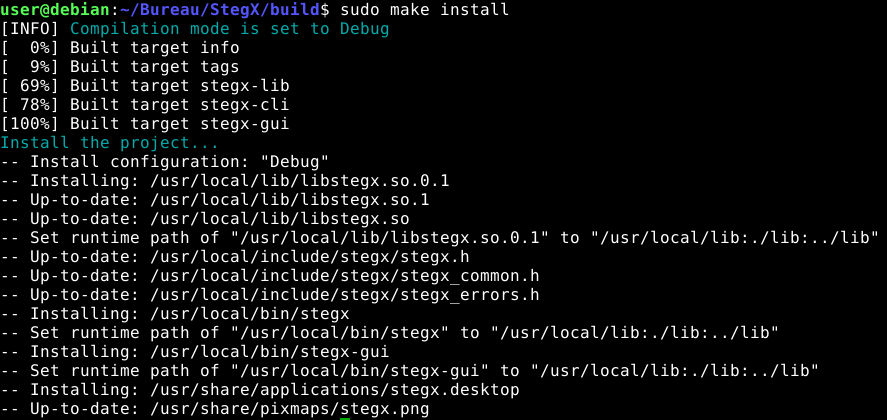
\includegraphics[scale=0.5]{pictures/install.png}

\underline{OU BIEN}

\begin{itemize}
\item Dans la section `Release`, télécharger le fichier `StegX-xxx.deb`.
\item Installer le en utilisant une interface à APT (par exemple en double cliquant
dessus), ou en utilisant la commande `sudo apt-get install ./StegX-xxx.deb`
depuis le répertoire de téléchargement.
\end{itemize}

\subsection{Désinstallation sous Linux}

Pour désinstaller StegX, taper dans sur le terminal : 
\begin{itemize}
\item sudo apt remove stegx
\end{itemize}

\subsection{Installation sous Windows}

\begin{itemize}
\item Aller sur https://www.github.com/Heisenberk/StegX/ et cliquer sur Release.
\item Télécharger l'archive et cliquer dessus à la fin du téléchargement.
\end{itemize}

\hspace{1cm}
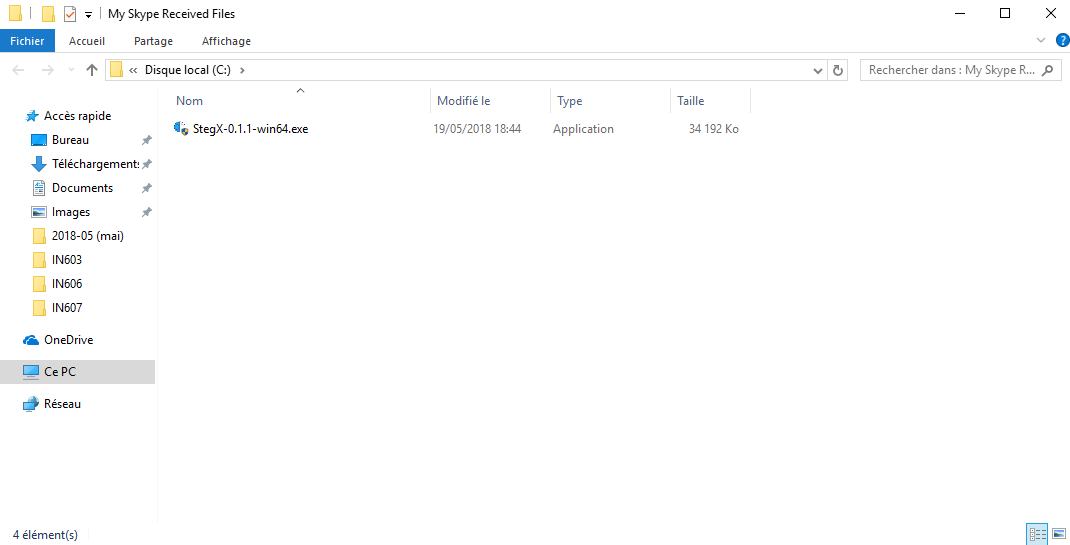
\includegraphics[scale=0.5]{pictures/ouverture.png}
\vspace{1cm}

\begin{itemize}
\item Cliquer sur "Suivant". 
\end{itemize}

\hspace{1cm}
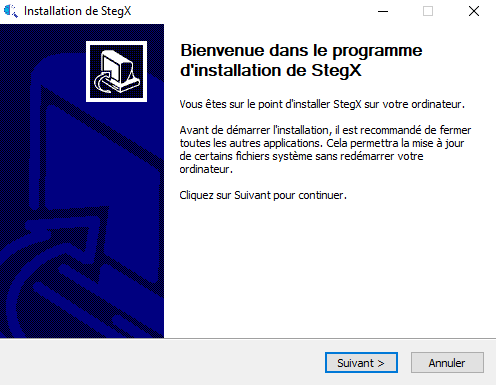
\includegraphics[scale=1]{pictures/presentation.png}
\vspace{1cm}

\begin{itemize}
\item Cliquer sur "J'accepte". 
\end{itemize}

\hspace{1cm}
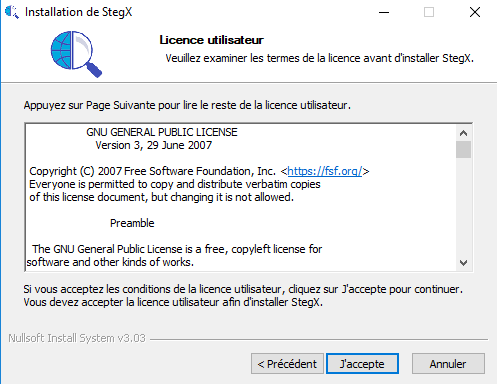
\includegraphics[scale=1]{pictures/licence.png}
\vspace{1cm}

\begin{itemize}
\item Cliquer sur "Suivant". 
\end{itemize}

\hspace{1cm}
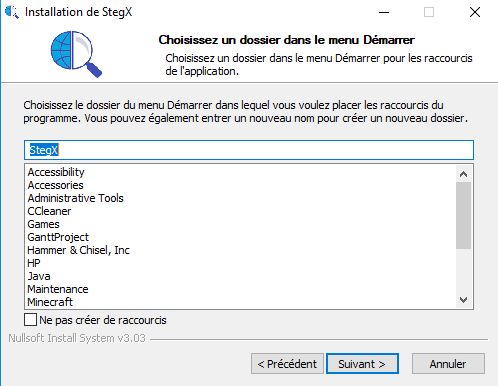
\includegraphics[scale=1]{pictures/debut.png}
\vspace{1cm}

\begin{itemize}
\item Sélectionner le premier choix. 
\item Cliquer sur "Suivant". 
\end{itemize}

\hspace{1cm}
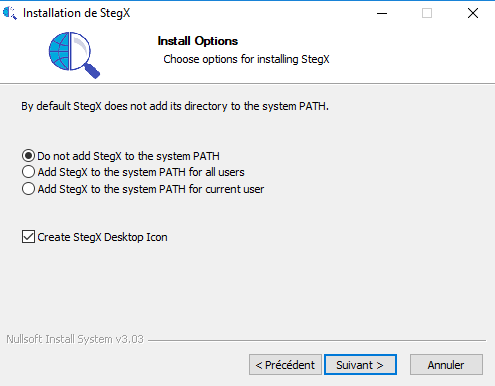
\includegraphics[scale=1]{pictures/path.png}
\vspace{1cm}

\begin{itemize}
\item Cliquer sur "Suivant". 
\end{itemize}

\hspace{1cm}
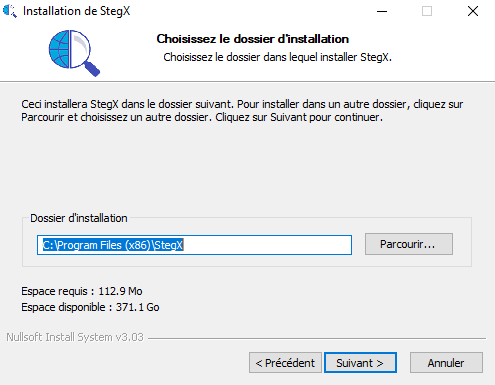
\includegraphics[scale=1]{pictures/taille.png}
\vspace{1cm}

\begin{itemize}
\item Choisir les composants de l'application à installer (interface 
en ligne de commande et/ou interface graphique). 
\end{itemize}

\hspace{1cm}
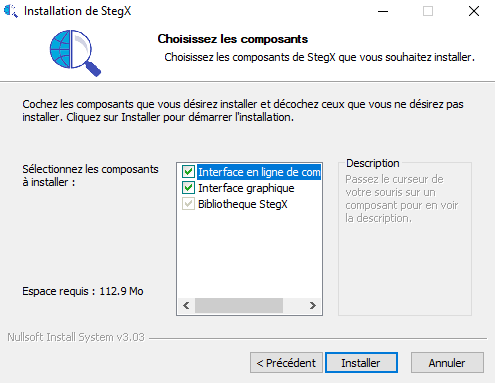
\includegraphics[scale=1]{pictures/choix.png}
\vspace{1cm}

\begin{itemize}
\item Choisir les composants de l'application à installer (interface 
en ligne de commande et/ou interface graphique). 
\item Cliquer sur "Suivant". 
\end{itemize}

\hspace{1cm}
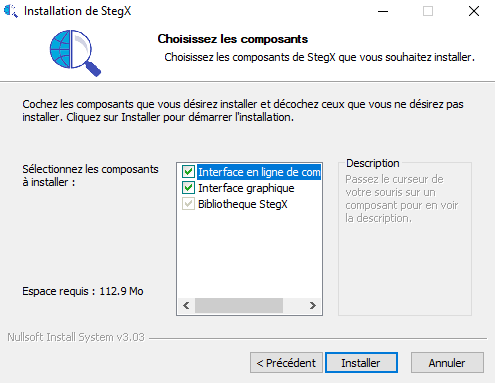
\includegraphics[scale=1]{pictures/choix.png}
\vspace{1cm}

\begin{itemize}
\item Attendre la fin de l'installation.
\item Cliquer sur "Suivant". 
\end{itemize}

\hspace{1cm}
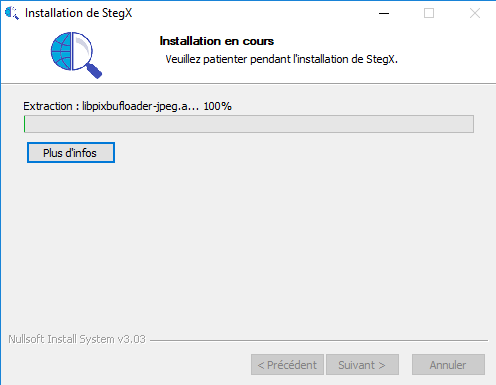
\includegraphics[scale=1]{pictures/installation.png}
\vspace{1cm}

\begin{itemize}
\item Cliquer sur "Fermer". 
\end{itemize}

\hspace{1cm}
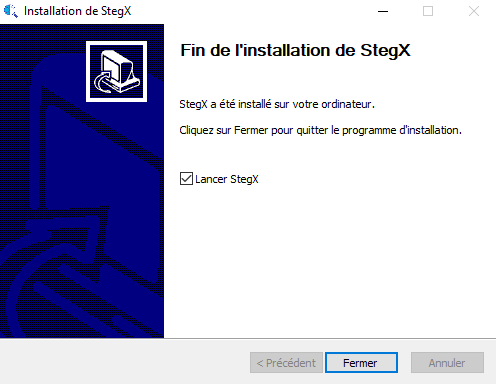
\includegraphics[scale=1]{pictures/fin.png}
\vspace{1cm}

\subsection{Désinstallation sous Windows}

\begin{itemize}
\item Accéder au panneau de configuration, cliquer sur désinstaller un programme,
sélectionner StegX et cliquer sur désinstaller.
\end{itemize}

\hspace{3cm}
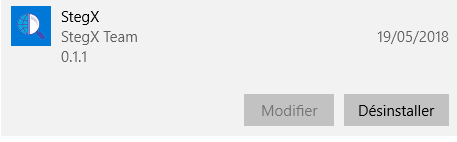
\includegraphics[scale=0.6]{pictures/desinstall.png}
\vspace{1cm}

\section{Manuel du développeur}

\section{Manuel de l'utilisateur}

\subsection{Interface en ligne de commande}

\subsection{Interface graphique}


\end{document}
